\begin{minipage}[t]{180mm}
\fcolorbox{black}{white}{
\begin{minipage}[b]{30mm}

\includegraphics[width=0.5\linewidth]{unflogo.pdf}
\end{minipage}
\begin{minipage}[b]{100mm}
\Huge \textbf{UNF NEWZ} \\
\Large -- Stadig uden nok søvn!
\end{minipage}
\begin{minipage}[b]{50mm}
\Large Fredag 19.07.2016 \\
\normalsize Redigeret i \LaTeX\ af \\ SOM, MGS
\end{minipage}
}
\end{minipage}



\begin{minipage}[b]{0.95\linewidth}
\begin{minipage}[t]{0.47\textwidth}
\vspace{1mm}
\section*{Dagens norske haikudikt}
\begin{center}
Sørlandssommer \\
smak av markjordbær \\
bak tynne blusser. \\
\emph{Geir Wigdel}
\end{center}
 

\section*{Ikke-kommutativ studenterrådgiv.}
\emph{Kære brevkasse}

En af mine venner siger, at for at være et godt menneske, skal man kunne se sig selv i øjnene. Er det derfor vampyrer og basiliker er så nederen?

\emph{Hilsen, en anonym stepdanser}

\subsection*{Svar}

Din ven har ret, for at være et godt menneske, skal man kunne se sig selv i øjnene. Dette kræver dog at ens øjne kan kigge på hinanden, hvilket ikke er fysiologisk muligt. Af denne grund er det eneste tidspunkt, det er muligt at se i sine egne øjne i dødsøjeblikket når sjælen forlader kroppen og i et kort øjeblik kigger på sig selv udefra. Enkelte indevider, der dør med åbne øjne, har i denne situation muligheden for at se i deres egne øjne, og helt rigtigt som din ven påpeger er det kun disse helt specielle mennesker vi ønsker at betegner som døde. 

Anden del af dit spørgsmål er dog en udbredt misforståelse, da hverken vamyrer eller basilisker er nederen. Vampyrer er som kendt fra sidste års nyheder den kvindelige, og ofte meget attraktive udgave af dataloger, og de er ofte mere nedringede end nederen, og har desuden yderst gode jobmuligheder i IT-konsulent-branchen. Vampyrer har desuden sjældent problemer med at kigge dem selv i øjnene, da de kan fjerne et af deres øjne fra den klassiske plads i hovedet, holde det i hånden og derved kigge i det andet øje, uden men der går ud over svage hovedpine på grund af den forstyrrede tredimensionale interpretation af omverdenen.

Basilisker er heller ikke, på nogen måde, nederen, men derimod nogle af de mest sympatiske skabinger, som kan kigge i deres egne øjne, ved at spejle sig i øjnene på deres døende ofre. Basilisker har desuden en vigtig betydning i økosystemet, da de fjerner aggresive helte og dumme princesser fra genpoolen og dermed øger befolkningens samlede kvalifikationer.

{\flushright\emph{Hilsen den ikke-kommutative studenterrådgivning}}

\end{minipage}%
\hfill\begin{minipage}[t]{0.47\textwidth}
\vspace{2mm}
\section*{Vejrudsigt}
\textbf{IMF, AU (fra DMI)}: Temperaturer fra 16 til 23 grader og skyet omkring middag med svag vind fra nordvest. Der forventes et moderat antal græspollen, og et lavt antal bynkepollen.

\textbf{Hogwarts}: Høj sandsynlighed for stjerneskud, og mange ugler på himlen, men der er set dementorer i skoven.

\section*{Fakta om Jylland}
Jylland er en halvø: den anden halvdel er immigreret til Mars, fordi de kom i krig over noget med en næse

\section*{Dagens matematiker}
Hvis du møder en matematiker, så sig noget sødt til hende/ham.

\section*{Dagens sandsynlighed}
Sandsynligheden for at der blandt $51$ er mindst $12$ elever der fordeles til ét kollegie er $1$. 

\section*{Hilsen}
Sune hilser Tobias mange gane fra Kirsten.
\vspace{2mm}
\emph{Bemærk at der hverken er morbiditeter eller seksuelle undertoner i ovenstående nyhed. Det beklager vi dyb, og lover bedring på morgfendagens dagsseddel. Vi fraråder generelt sober kommunikation mellem personer, da vi anser dette for trættende, men det er desværre kun den ældre halvdel af redaktionen der der ufejlbart.}
\end{minipage}

\begin{center}
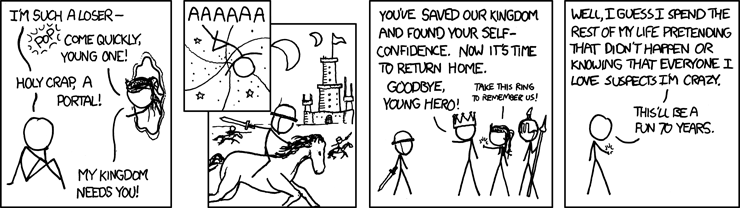
\includegraphics[width=\linewidth]{childrens_fantasy.png}
\tiny Randall Munroe, http://xkcd.com/693/, CC-BY-SA-2.5

\tiny UNF Newz er avisen hvor at ansvarshavende redaktør fralægger sig ethvert ansvar for eventuel plagiering, kaniner, tysk, stavefelj, kaffe, dårlig humor, glemsomhed, katte, store sigmaer, pile, skyer, dårlige oversættelser og alt hvad eventuelle homo sapiens sapiens kunne finde på at holde imod UNF Newz! Dog tager UNF Newz fuld credit og copyright for alle guldkorn, magickort, mus, \TeX, humor, smil, Mortener, kaffe, før-fremtid, ringe og/eller Rubiksterning.
\end{center}
\end{minipage}

